
\subsection{Processing of relative clauses}
\begin{figure*}[t]
\centering
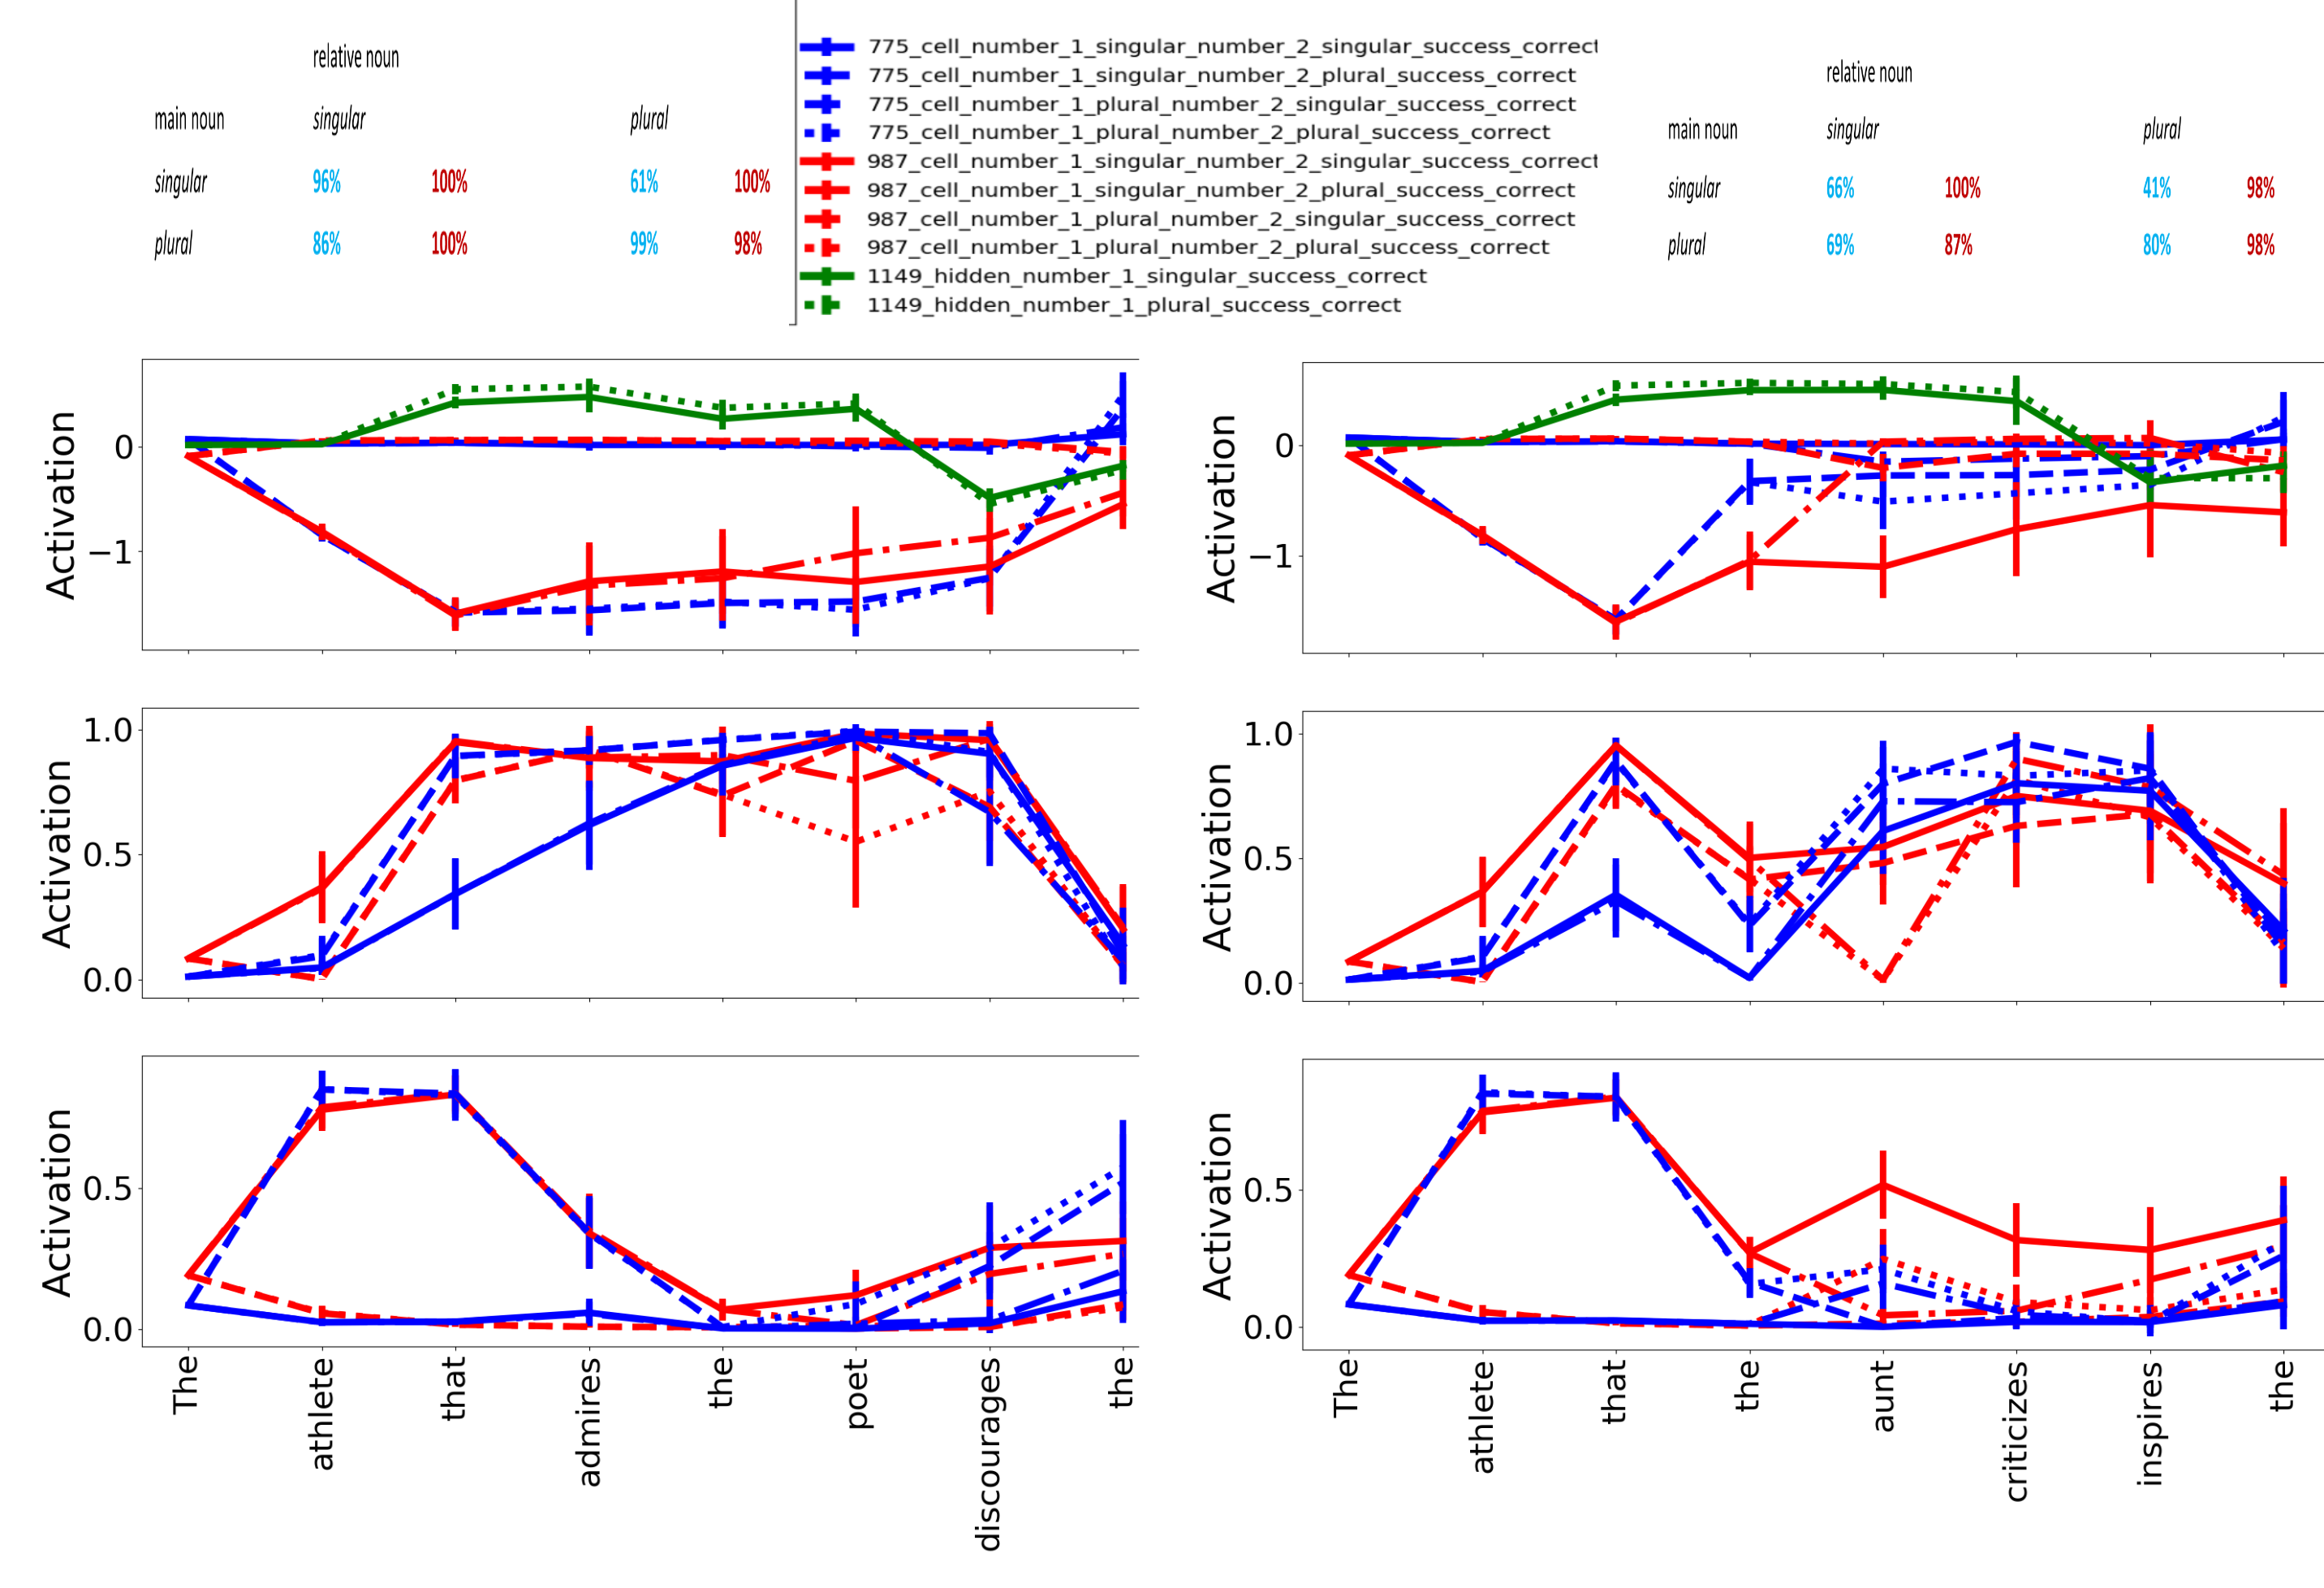
\includegraphics[width=\textwidth]{Figures/Figure8_RC.png}
\caption{Subject-verb agreement in relative clauses: agreement-task accuracy for (A) subject relatives and (B) object relatives. (C \& D) The corresponding cell activations for the number units (775 and 987) and the syntax unit 1149. (E \& F) The corresponding forget-gate activity and (G \& H) input-gate activity of the number units. }
\end{figure*}

\begin{figure}[b]
\centering
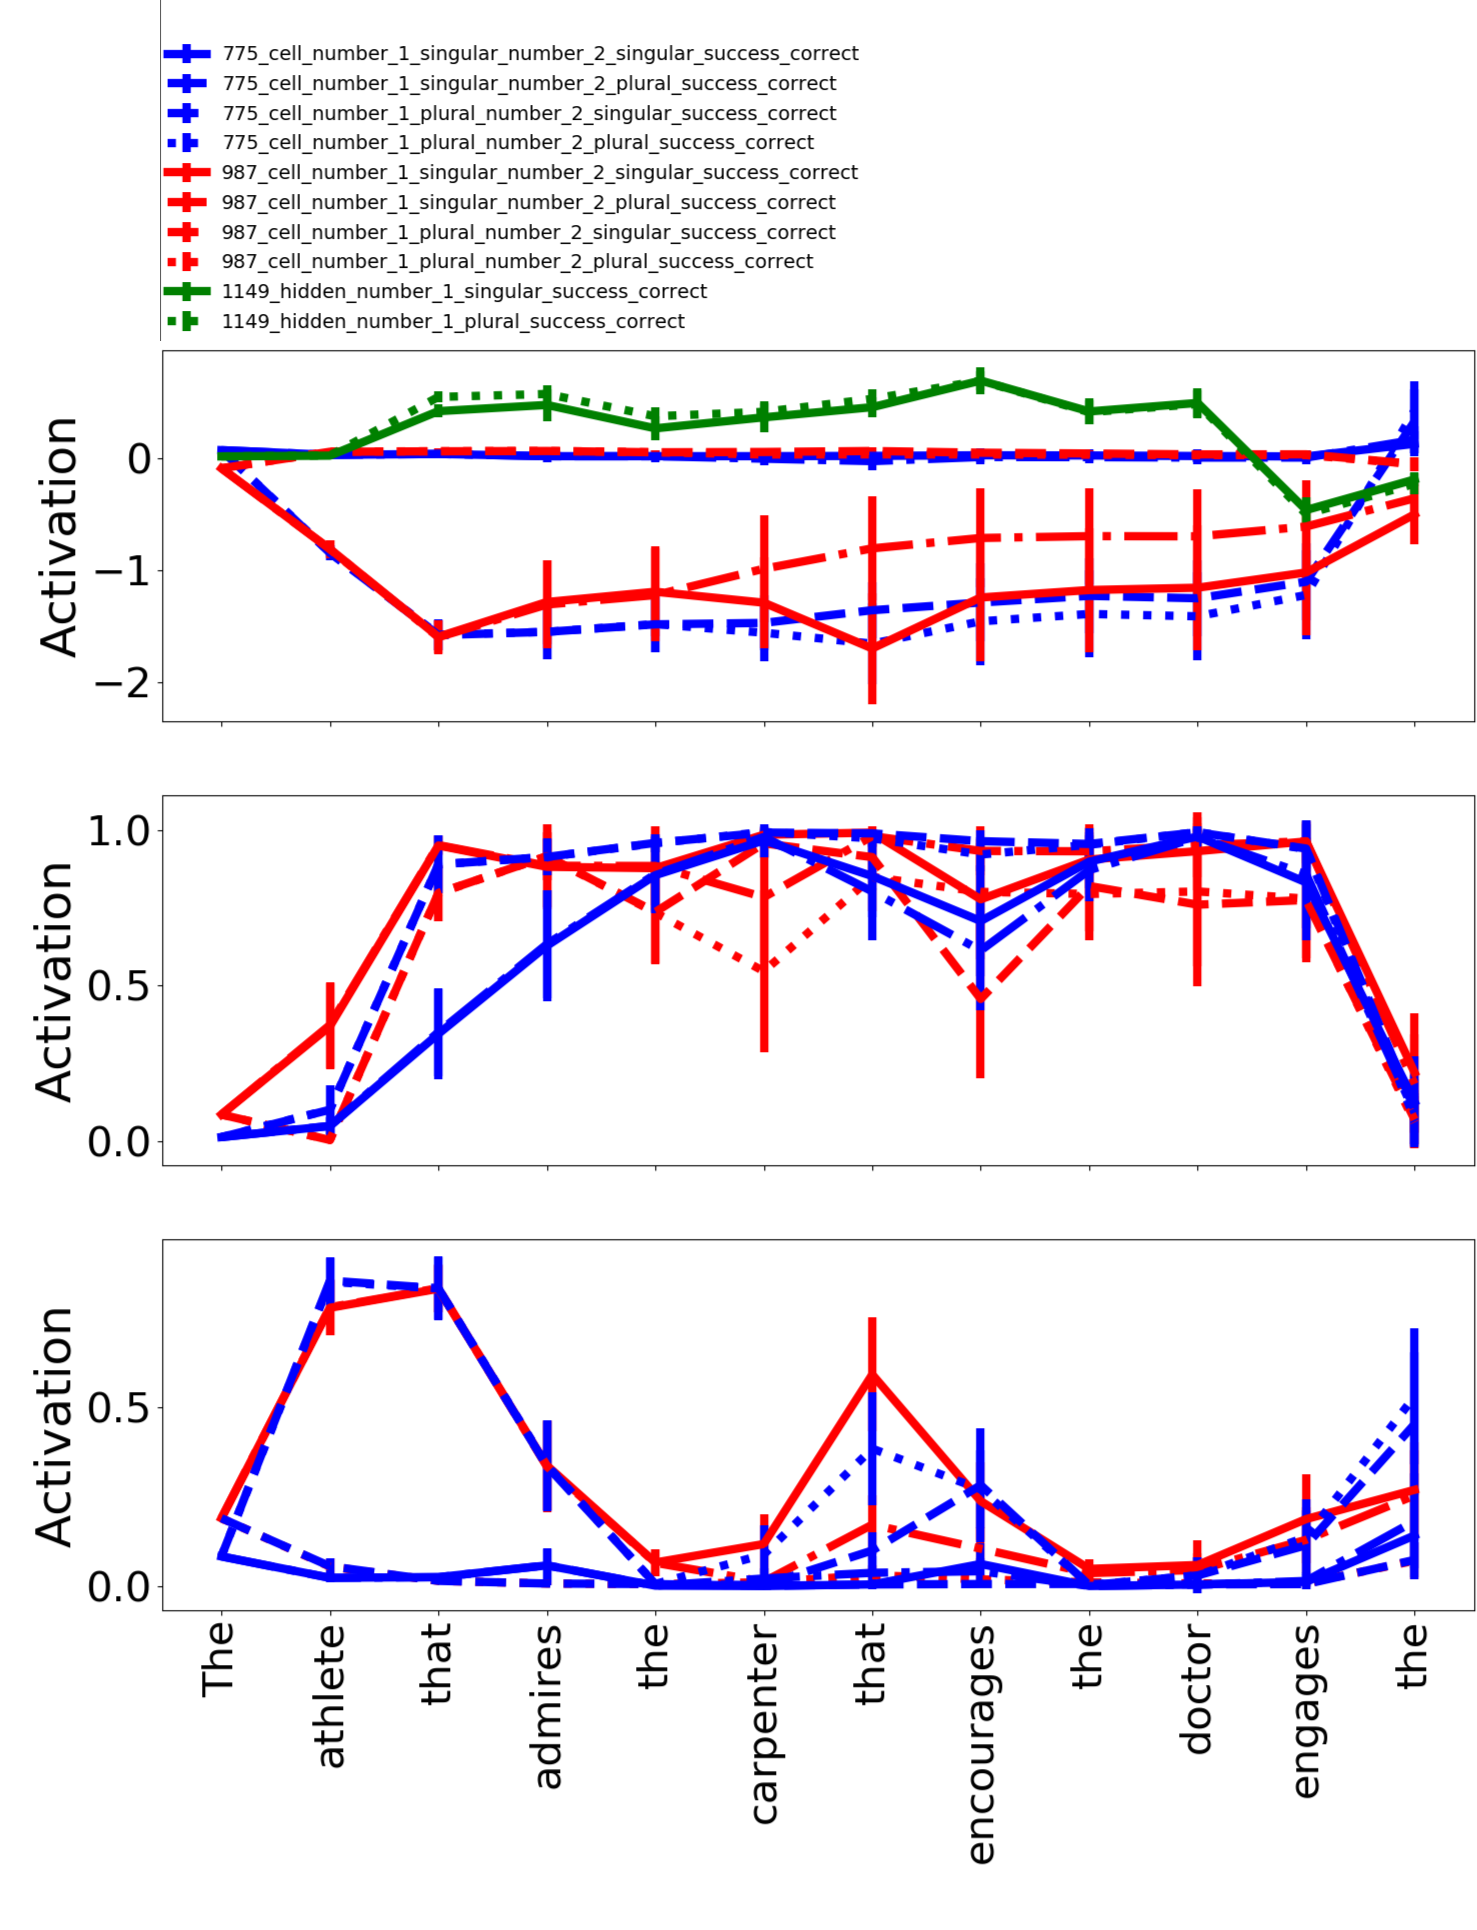
\includegraphics[width=\linewidth]{Figures/Figure9_doubleRC.png}
\caption{Processing of subject relatives with double embeddings. (A) Cell activity of the number and syntax units (775, 987 and 1149) (B) The corresponding forget-gate and (C) input-gate activity.}
\end{figure}

Sentences with relative clauses (RCs) and their processing are of major interset in linguistic and psycholinguistic (cite) given that they involve embedding, syntactic movement (object relatives)...and require theoretical...\textcolor{red}{complete this introductory sentence about RCs}. This section explores the dynamics of the LR-number units and syntax unit 1150 during the processing of sentences with RCs. Specifically, we looked into number agreement during the processing of subject and object relatives, the latter of which is known to be more prone for errors in humans (cite). In particular, we analyzed the performance of the network on the NA-task and compared it to the underlying gate dynamics of the LR-number units, similarly to the nounPP case in section 5.1. 

Figure X shows the behavioral results of the network on the subjrel (panel A) and objrel (panel B) NA-tasks. Network performance on the subjrel NA-task was relatively high compared to the objrel task, in both the congruent (main diagonal) and incongruent cases (off-diagonal values) \textcolor{red}{requires quantification}. This matches human performance on similar tasks (cite) and extends the analysis of previously reported results on the processing of RCs by LSTM-LM (Linzen 2018). Interestingly, when the subject is singular, more errors are made by human participants compared to the plural case (Bock). This matches LSTM-LM performance in both subjrel and objrel tasks and in both congurent and incongruent cases: $ACC^subjrel_{SS}<ACC^subjrel_{SP}, ACC^subjrel_{SP}<ACC^subjrel_{PS}, ACC^objrel{SS}<ACC^objrel{SP}, ACC^objrel{SP}<ACC^objrel{PS}$. Given that the language model was trained on word tokens, these results suggest that the source for the singular-plural assymetry resides at the word-level statistics in the corpus and not at the segmental level (cite Miller and Bock), also for humans.

and the corresponding gate dynamics during the processing of the sentences (panels C and D, respectively).


To explore thduring the processing of sentences with two embedded subject-relatuve clauses (double-subjrel). 
